% ============================================================
%  FLBL2 System Architecture -- Research-paper TikZ diagram
%  Compile:  pdflatex flbl2_architecture.tex
%            xelatex  flbl2_architecture.tex
% ============================================================
\documentclass[tikz, border=12pt]{standalone}

\usepackage{tikz}
\usepackage{xcolor}
\usepackage{amsmath,amssymb}

\usetikzlibrary{arrows.meta, positioning, calc, backgrounds, fit}

% ----- colour palette ----------------------------------------
\definecolor{CEdge}   {HTML}{1A6FB5}
\definecolor{CEdgeLt} {HTML}{D6E8F7}
\definecolor{CSrv}    {HTML}{1B7A3E}
\definecolor{CSrvLt}  {HTML}{D4EDDA}
\definecolor{CIPFS}   {HTML}{C05A00}
\definecolor{CIPFSLt} {HTML}{FDE8CF}
\definecolor{CChain}  {HTML}{5B2D8E}
\definecolor{CChainLt}{HTML}{EAD9F8}
\definecolor{CGray}   {HTML}{555555}
\definecolor{CBg}     {HTML}{F4F6F9}

% Step-number macro: [N] in bold gray -- NO \tikz inside, safe in nodes
\newcommand{\sn}[1]{%
  {\sffamily\bfseries\textcolor{CGray}{[\,#1\,]}}%
}

% ----- reusable styles ----------------------------------------
\tikzset{
  >=Latex,
  % Arrow label box
  annot/.style={
    font=\scriptsize\sffamily,
    fill=white,
    draw=CGray!45,
    rounded corners=2pt,
    inner sep=2pt
  },
  % Coloured background panel  (single-arg: colour name)
  mypanel/.style={
    rounded corners=6pt,
    draw=#1,
    fill=#1!12,
    line width=1.2pt
  },
  % Component inner box  (single-arg: border colour)
  mybox/.style={
    rounded corners=4pt,
    draw=#1,
    fill=white,
    line width=0.85pt,
    align=center,
    inner sep=5pt,
    text width=3.3cm
  },
}

% =============================================================
\begin{document}
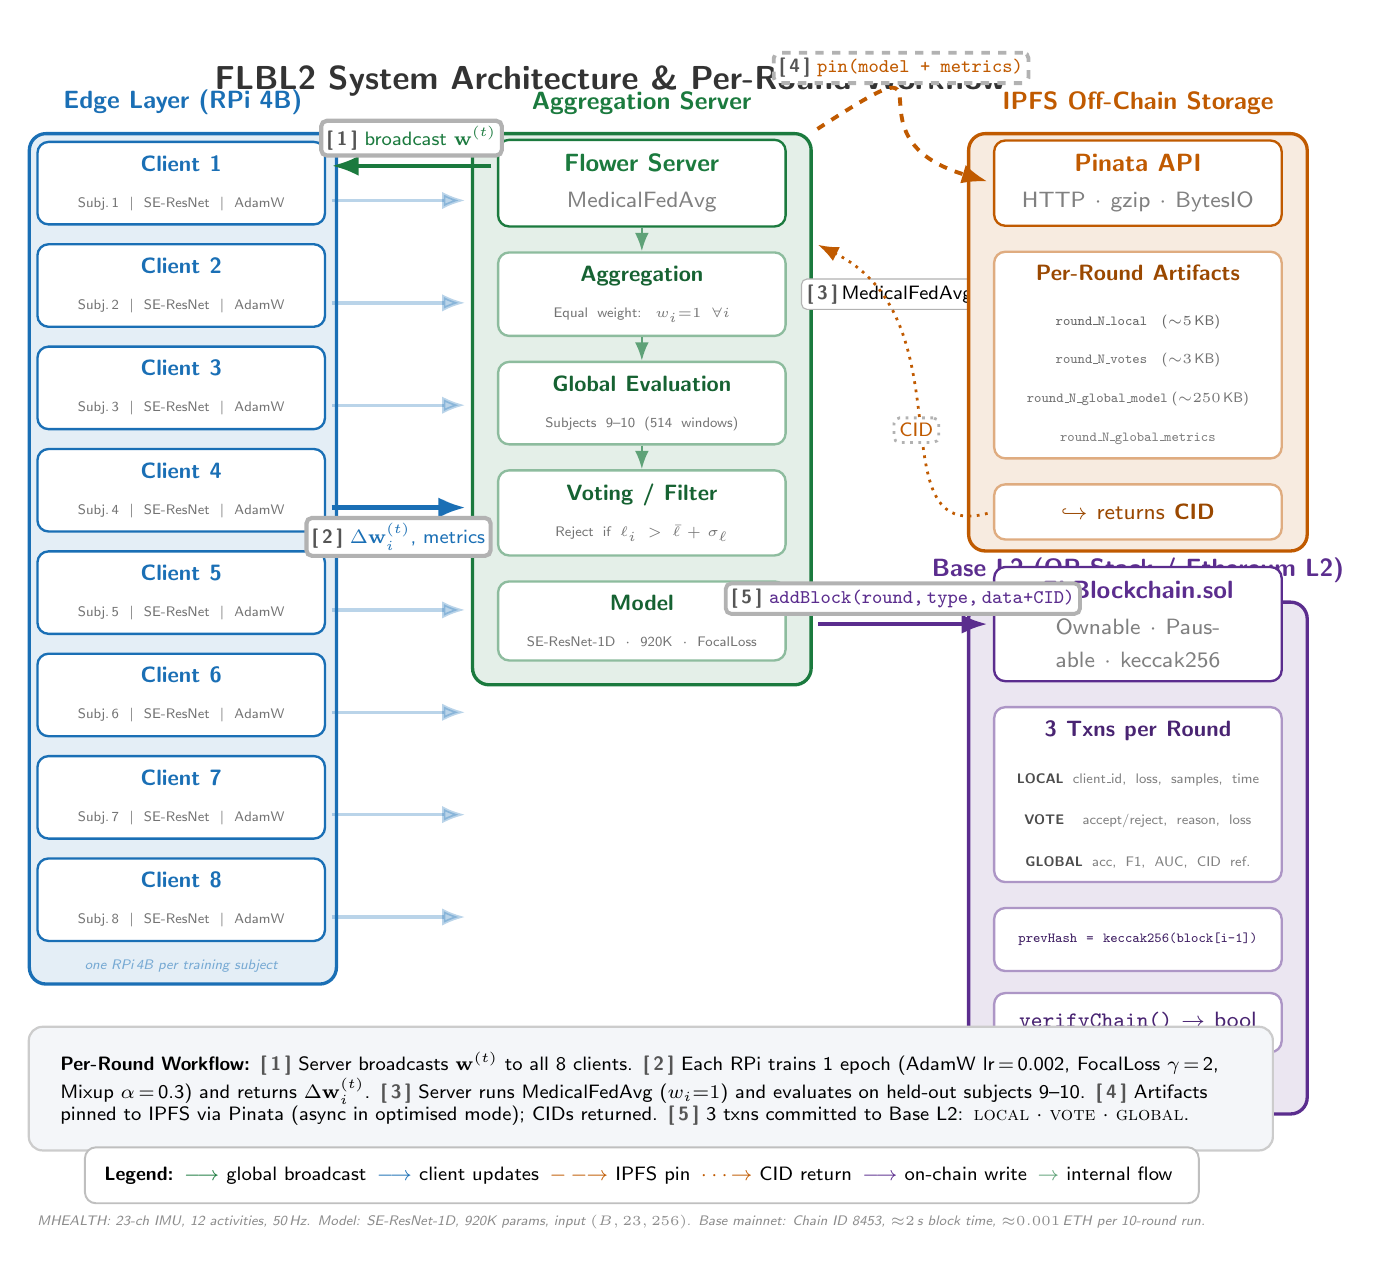
\begin{tikzpicture}[font=\sffamily]

% ── TITLE ─────────────────────────────────────────────────────
\node[font=\large\bfseries\sffamily, text=black!80]
  (title) at (7.4, 1.8)
  {FLBL2 System Architecture \& Per-Round Workflow};

% ── EDGE CLIENTS PANEL ────────────────────────────────────────
%  8 clients at y = 0.5, -0.8, -2.1, ... (-1.3 cm spacing)

\node[mypanel=CEdge, minimum width=3.9cm, minimum height=10.8cm,
      anchor=north west] (cpanel) at (0, 1.15) {};
\node[font=\small\bfseries\sffamily, text=CEdge,
      above=0.1cm of cpanel.north, anchor=south]
  {\textsc{Edge Layer (RPi 4B)}};

% Client 1
\node[mybox=CEdge, minimum height=0.85cm] (c1) at (1.95,  0.5) {
  {\footnotesize\textcolor{CEdge}{\textbf{Client 1}}}\\[1pt]
  {\tiny\textcolor{black!55}{Subj.\,1 $|$ SE-ResNet $|$ AdamW}}
};
% Client 2
\node[mybox=CEdge, minimum height=0.85cm] (c2) at (1.95, -0.8) {
  {\footnotesize\textcolor{CEdge}{\textbf{Client 2}}}\\[1pt]
  {\tiny\textcolor{black!55}{Subj.\,2 $|$ SE-ResNet $|$ AdamW}}
};
% Client 3
\node[mybox=CEdge, minimum height=0.85cm] (c3) at (1.95, -2.1) {
  {\footnotesize\textcolor{CEdge}{\textbf{Client 3}}}\\[1pt]
  {\tiny\textcolor{black!55}{Subj.\,3 $|$ SE-ResNet $|$ AdamW}}
};
% Client 4
\node[mybox=CEdge, minimum height=0.85cm] (c4) at (1.95, -3.4) {
  {\footnotesize\textcolor{CEdge}{\textbf{Client 4}}}\\[1pt]
  {\tiny\textcolor{black!55}{Subj.\,4 $|$ SE-ResNet $|$ AdamW}}
};
% Client 5
\node[mybox=CEdge, minimum height=0.85cm] (c5) at (1.95, -4.7) {
  {\footnotesize\textcolor{CEdge}{\textbf{Client 5}}}\\[1pt]
  {\tiny\textcolor{black!55}{Subj.\,5 $|$ SE-ResNet $|$ AdamW}}
};
% Client 6
\node[mybox=CEdge, minimum height=0.85cm] (c6) at (1.95, -6.0) {
  {\footnotesize\textcolor{CEdge}{\textbf{Client 6}}}\\[1pt]
  {\tiny\textcolor{black!55}{Subj.\,6 $|$ SE-ResNet $|$ AdamW}}
};
% Client 7
\node[mybox=CEdge, minimum height=0.85cm] (c7) at (1.95, -7.3) {
  {\footnotesize\textcolor{CEdge}{\textbf{Client 7}}}\\[1pt]
  {\tiny\textcolor{black!55}{Subj.\,7 $|$ SE-ResNet $|$ AdamW}}
};
% Client 8
\node[mybox=CEdge, minimum height=0.85cm] (c8) at (1.95, -8.6) {
  {\footnotesize\textcolor{CEdge}{\textbf{Client 8}}}\\[1pt]
  {\tiny\textcolor{black!55}{Subj.\,8 $|$ SE-ResNet $|$ AdamW}}
};
\node[font=\tiny\sffamily\itshape, text=CEdge!60, below=3pt of c8]
  {one RPi\,4B per training subject};

% ── AGGREGATION SERVER PANEL ───────────────────────────────────
\node[mypanel=CSrv, minimum width=4.3cm, minimum height=7.0cm,
      anchor=north] (spanel) at (7.8, 1.15) {};
\node[font=\small\bfseries\sffamily, text=CSrv,
      above=0.1cm of spanel.north, anchor=south]
  {\textsc{Aggregation Server}};

\node[mybox=CSrv, minimum height=1.1cm] (flsrv) at (7.8, 0.5) {
  {\small\textcolor{CSrv}{\textbf{Flower Server}}}\\[1pt]
  {\footnotesize\textcolor{black!50}{MedicalFedAvg}}
};
\node[mybox=CSrv!50, minimum height=0.85cm, below=0.3cm of flsrv] (aggbox) {
  {\footnotesize\textbf{\textcolor{CSrv!80!black}{Aggregation}}}\\[1pt]
  {\tiny\textcolor{black!55}{Equal weight: $w_i{=}1\;\forall i$}}
};
\node[mybox=CSrv!50, minimum height=0.85cm, below=0.3cm of aggbox] (evalbox) {
  {\footnotesize\textbf{\textcolor{CSrv!80!black}{Global Evaluation}}}\\[1pt]
  {\tiny\textcolor{black!55}{Subjects 9--10 (514 windows)}}
};
\node[mybox=CSrv!50, minimum height=0.85cm, below=0.3cm of evalbox] (votebox) {
  {\footnotesize\textbf{\textcolor{CSrv!80!black}{Voting / Filter}}}\\[1pt]
  {\tiny\textcolor{black!55}{Reject if $\ell_i > \bar{\ell} + \sigma_{\ell}$}}
};
\node[mybox=CSrv!50, minimum height=0.85cm, below=0.3cm of votebox] (mdlbox) {
  {\footnotesize\textbf{\textcolor{CSrv!80!black}{Model}}}\\[1pt]
  {\tiny\textcolor{black!55}{SE-ResNet-1D $\cdot$ 920K $\cdot$ FocalLoss}}
};

% Internal server flow arrows
\draw[->, line width=0.8pt, color=CSrv!70] (flsrv.south)  -- (aggbox.north);
\draw[->, line width=0.8pt, color=CSrv!70] (aggbox.south)  -- (evalbox.north);
\draw[->, line width=0.8pt, color=CSrv!70] (evalbox.south) -- (votebox.north);

% Step 3 annotation
\node[annot, right=0.18cm of aggbox]
  {\sn{3}\,MedicalFedAvg};

% ── IPFS PANEL ────────────────────────────────────────────────
\node[mypanel=CIPFS, minimum width=4.3cm, minimum height=5.3cm,
      anchor=north] (ipanel) at (14.1, 1.15) {};
\node[font=\small\bfseries\sffamily, text=CIPFS,
      above=0.1cm of ipanel.north, anchor=south]
  {\textsc{IPFS Off-Chain Storage}};

\node[mybox=CIPFS, minimum height=1.0cm] (pinata) at (14.1, 0.5) {
  {\small\textcolor{CIPFS}{\textbf{Pinata API}}}\\[1pt]
  {\footnotesize\textcolor{black!50}{HTTP $\cdot$ gzip $\cdot$ BytesIO}}
};

% Multi-line artifact box -- each \\ is OUTSIDE every \textcolor group
\node[mybox=CIPFS!50, minimum height=2.4cm, below=0.3cm of pinata] (artbox) {
  {\footnotesize\textbf{\textcolor{CIPFS!80!black}{Per-Round Artifacts}}}\\[4pt]
  {\tiny\textcolor{black!60}{\texttt{round\_N\_local}\quad(${\sim}5$\,KB)}}\\[2pt]
  {\tiny\textcolor{black!55}{\texttt{round\_N\_votes}\quad(${\sim}3$\,KB)}}\\[2pt]
  {\tiny\textcolor{black!55}{\texttt{round\_N\_global\_model}\;(${\sim}250$\,KB)}}\\[2pt]
  {\tiny\textcolor{black!50}{\texttt{round\_N\_global\_metrics}}}
};

\node[mybox=CIPFS!50, minimum height=0.7cm, below=0.3cm of artbox] (cidout) {
  {\footnotesize\textcolor{CIPFS!80!black}{$\hookrightarrow$ returns \textbf{CID}}}
};

% ── BASE L2 PANEL ─────────────────────────────────────────────
\node[mypanel=CChain, minimum width=4.3cm, minimum height=6.5cm,
      anchor=north] (bpanel) at (14.1, -4.8) {};
\node[font=\small\bfseries\sffamily, text=CChain,
      above=0.1cm of bpanel.north, anchor=south]
  {\textsc{Base L2 (OP Stack / Ethereum L2)}};

\node[mybox=CChain, minimum height=1.0cm] (solidity) at (14.1, -5.1) {
  {\small\textcolor{CChain}{\textbf{FLBlockchain.sol}}}\\[1pt]
  {\footnotesize\textcolor{black!50}{Ownable $\cdot$ Pausable $\cdot$ keccak256}}
};

% Block types -- each \\ is OUTSIDE every \textcolor group
\node[mybox=CChain!50, minimum height=2.2cm, below=0.3cm of solidity] (btypes) {
  {\footnotesize\textbf{\textcolor{CChain!80!black}{3 Txns per Round}}}\\[5pt]
  {\tiny\textbf{\textcolor{black!70}{LOCAL}}}~{\tiny\textcolor{black!50}{client\_id, loss, samples, time}}\\[3pt]
  {\tiny\textbf{\textcolor{black!70}{VOTE}}}~~{\tiny\textcolor{black!50}{accept/reject, reason, loss}}\\[3pt]
  {\tiny\textbf{\textcolor{black!70}{GLOBAL}}}~{\tiny\textcolor{black!50}{acc, F1, AUC, CID ref.}}
};

\node[mybox=CChain!50, minimum height=0.8cm, below=0.3cm of btypes] (hashchain) {
  {\tiny\textcolor{CChain!70!black}{\texttt{prevHash = keccak256(block[i-1])}}}
};
\node[mybox=CChain!50, minimum height=0.75cm, below=0.25cm of hashchain] (verifybox) {
  {\footnotesize\textcolor{CChain!80!black}{\texttt{verifyChain()} $\to$ bool}}
};

% ── ARROWS ────────────────────────────────────────────────────

% (1) Server --> Clients: broadcast global weights  (upper lane)
\draw[->, line width=1.5pt, color=CSrv, shorten >=2pt, shorten <=2pt]
  ($(flsrv.west)+(0,+0.22)$) -- ($(c1.east)+(0,+0.22)$)
  node[annot, midway, above=3pt]
    {\sn{1} broadcast $\mathbf{w}^{(t)}$};

% (2) Clients --> Server: local updates  (lower lane, faint x8, one labeled)
\foreach \ci in {c1,c2,c3,c4,c5,c6,c7,c8}{
  \draw[->, line width=1.2pt, color=CEdge, opacity=0.30,
        shorten >=2pt, shorten <=2pt]
    ($(\ci.east)+(0,-0.22)$) -- ($(spanel.west |- \ci)+(0,-0.22)$);
}
% labeled return arrow at c4
\draw[->, line width=1.5pt, color=CEdge, shorten >=2pt, shorten <=2pt]
  ($(c4.east)+(0,-0.22)$) -- ($(spanel.west |- c4)+(0,-0.22)$)
  node[annot, midway, below=3pt]
    {\sn{2} $\Delta\mathbf{w}_i^{(t)}$, metrics};

% (4) Server --> IPFS: pin artifacts (curved dashed orange)
\draw[->, line width=1.4pt, color=CIPFS, dashed,
      shorten >=2pt, shorten <=2pt]
  (spanel.north east) .. controls +(2.0,1.3) and +(-2.0,0.6) .. (pinata.west)
  node[annot, pos=0.45, above=4pt]
    {\sn{4} \texttt{pin(model + metrics)}};

% CID return (curved dotted orange)
\draw[->, line width=1.0pt, color=CIPFS, dotted,
      shorten >=2pt, shorten <=2pt]
  (cidout.west) .. controls +(-1.5,-0.4) and +(2.0,-1.0) ..
  ($(spanel.north east)+(0,-1.4)$)
  node[annot, pos=0.52, below=2pt]
    {CID};

% (5) Server --> Base L2: addBlock  (horizontal solid purple)
\draw[->, line width=1.4pt, color=CChain, shorten >=2pt, shorten <=2pt]
  ($(spanel.east |- solidity)$) -- (solidity.west)
  node[annot, midway, above=3pt]
    {\sn{5} \texttt{addBlock(round,\,type,\,data+CID)}};

% ── WORKFLOW BANNER ───────────────────────────────────────────
\node[rounded corners=5pt, fill=CBg, draw=black!20, line width=0.8pt,
      minimum width=15.8cm, text width=15.0cm,
      anchor=north west, inner sep=9pt,
      font=\scriptsize\sffamily, align=left]
  (banner) at (0, -10.2) {
  \textbf{Per-Round Workflow:}\enspace
  \sn{1}~Server broadcasts $\mathbf{w}^{(t)}$ to all 8 clients.\enspace
  \sn{2}~Each RPi trains 1 epoch (AdamW lr\,=\,0.002, FocalLoss $\gamma$\,=\,2,
  Mixup $\alpha$\,=\,0.3) and returns $\Delta\mathbf{w}_i^{(t)}$.\enspace
  \sn{3}~Server runs MedicalFedAvg ($w_i{=}1$) and evaluates on held-out subjects 9--10.\enspace
  \sn{4}~Artifacts pinned to IPFS via Pinata (async in optimised mode); CIDs returned.\enspace
  \sn{5}~3 txns committed to Base L2: \textsc{local} $\cdot$ \textsc{vote} $\cdot$ \textsc{global}.
};

% ── LEGEND ────────────────────────────────────────────────────
\node[rounded corners=4pt, fill=white, draw=black!25, line width=0.7pt,
      inner sep=7pt, font=\scriptsize\sffamily, align=left]
  (legend) at (7.8, -12.1) {
  \textbf{Legend:}\enspace
  {\color{CSrv}$\longrightarrow$}~global broadcast\enspace
  {\color{CEdge}$\longrightarrow$}~client updates\enspace
  {\color{CIPFS}$-\,-\!\!\to$}~IPFS pin\enspace
  {\color{CIPFS}$\cdots\!\to$}~CID return\enspace
  {\color{CChain}$\longrightarrow$}~on-chain write\enspace
  {\color{CSrv!70}$\rightarrow$}~internal flow
};

% ── FOOTER NOTE ───────────────────────────────────────────────
\node[font=\tiny\sffamily\itshape, text=black!45, anchor=south west]
  at (0, -12.9) {
  MHEALTH: 23-ch IMU, 12 activities, 50\,Hz.\enspace
  Model: SE-ResNet-1D, 920K params, input $(B,23,256)$.\enspace
  Base mainnet: Chain ID~8453, ${\approx}2$\,s block time,
  ${\approx}0.001$\,ETH per 10-round run.
};

\end{tikzpicture}
\end{document}
